\documentclass[a4paper,11pt]{report}

\usepackage{fullpage}

\usepackage{amsmath}
\usepackage{bussproofs}
\usepackage{mathpartir}
\usepackage{prooftrees}
\usepackage{placeins}
\usepackage{color}

% Minted
\usepackage[cache=false]{minted}

\newmintinline{c}{
  fontsize=\small,
  breaklines=true
}

\newminted{c}{
  frame=single,
  framesep=2mm,
  fontsize=\scriptsize,
  mathescape
}

\newminted[clinecode]{c}{
  frame=single,
  framesep=2mm,
  fontsize=\scriptsize,
  mathescape,
  linenos
}

\newcommand*{\BBox}[1]{\draw (#1 + 0.5,0.5) -- (#1 + 1.5,0.5) -- (#1 + 1.5,-0.2)
  -- (#1 + 0.5,-0.2) -- cycle;}
\newcommand*{\SBox}[1]{}

\newcommand*{\equal}{=}

% for finite state automata
\usepackage{tikz}
\usetikzlibrary{automata,positioning}

\author{Sylvain Julmy}
\date{\today}

\setlength{\parindent}{0pt}

\begin{document}

\begin{center}
  \Large{
    System-oriented Programming\\
    Spring 2018
  }
  
  \noindent\makebox[\linewidth]{\rule{\linewidth}{0.4pt}}
  S04
  \noindent\makebox[\linewidth]{\rule{\linewidth}{0.4pt}}

  \begin{flushleft}
    Professor : Philippe Cudré-Mauroux

    Assistant : Michael Luggen
  \end{flushleft}
  
  \noindent\makebox[\linewidth]{\rule{\linewidth}{0.4pt}}

  Submitted by Sylvain Julmy
  
  \noindent\makebox[\linewidth]{\rule{\textwidth}{1pt}}
\end{center}

Note : the complete source file are available inside the zipped file.

\section*{Exercise 1}

When we try to add an external variable of type \verb+char+ $c$, we got a
compilation error when trying to linking (with \verb+ld+) the object code,
because the variable $c$ don't exists.

We simply modify the source of \verb+global2.c+ by adding the following line in
the code :

\begin{ccode}
char c;
\end{ccode}

Then the compilation is succesfull because the linker have found the variable
$c$ in the object code.

\section*{Exercise 2}

\subsection*{a)}

Figures~\ref{fig:ex4-a} shows the flow of the function call.

\begin{figure}[ht]
  \centering
  \frame{
    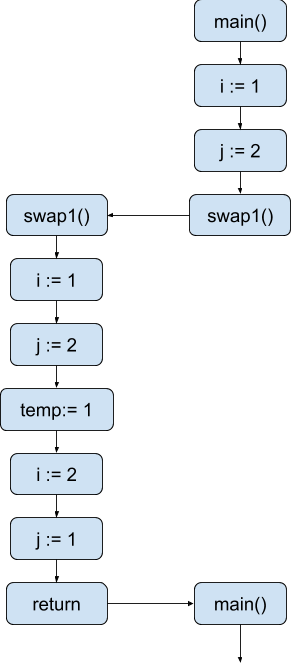
\includegraphics[width=0.25\textwidth]{figures/SOP_s04_ex2_a}
  }
  \caption{\label{fig:ex4-a} Flow of the function calls from Example 1 of GDB tutorial.}
\end{figure}

Figures~\ref{fig:ex4-a-ast} shows the AST of the function call, note that the
declaration of the variable are normally not part of the AST because they are
erase by the compiler because they are not allocated at runtime. They are here
for information about the program.

\begin{figure}[ht]
  \centering
  \begin{forest}
    [main
    [$int\ i; int\ j;$
    [list of statement
    [$\equal$ [$\&i$] [$1$]]
    [$\equal$ [$\&j$] [$2$]]
    [$functionCall(swap1)$
    [arguments [$i \equal 1;$][$j \equal 2;$]]
    [$int\ temp;$
    [list of statement
    [$\equal$ [$\&temp$][$\&i$]]
    [$\equal$ [$\&i$][$\&j$]]
    [$\equal$ [$\&j$][$\&temp$]]
    ]    ]    ]    ]    ]    ]
  \end{forest}
  \caption{\label{fig:ex4-a-ast}AST of the function main.}
\end{figure}

\FloatBarrier

\subsection*{b)}

We use the following list of gdb command :

\begin{verbatim}
// breakpoint at function swap1
br swap1
// breakpoint before returning from swap1
br 7
run

// display the variables
display i
display j
display temp

// display the arguments of stack1
frame 0

// continue to next breakpoint
c
// the value of i and j has been exchanged inside the function
n
// display the variables
display i
display j
// value hasn't been exchanged
\end{verbatim}

The value of the variables are not exchanged, because the function $swap1$ is a
call-by-value function and the value of $i$ and $j$ are copied on the stack. We
have to use pointer in order to have a call-by-reference argument.

\section*{Exercise 3}

\subsection*{a)}

The macro definition is wrong because of the precedence of the operators in C.
For example, if the use \cinline|square(4 + 1)|, this would expand to
\cinline|4 + 1 * 4 + 1|, which would lead to an unexpected result. So we have to
write the macro like the following :

\begin{ccode}
#define square(x) ((x) * (x))
\end{ccode}

\subsection*{b)}

\begin{ccode}
// PRE : x and y are variable identifier of type Type
#define swap(x, y, Type) do{Type t = x; x=y;y=t;}while(0);
\end{ccode}

\subsection*{c)}

Well, I do know the trick about using a \cinline+do while+ construction in order
to prevent bug...

The idea is to prevent unexpected statement precedence by using the mentionned
construction. This does not affect the compiler because the code is simply
erased by the compiler because the \cinline+do while+ does nothing.


\section*{Exercise 4}

\subsection*{a)}
\begin{forest}
  [$hello$
  [$hello.o$ [$hello.c$]]
  [$tellMe.o$ [$tellMe.c$]]
  ]
\end{forest}

\subsection*{b)}

Note : the warnings generated by the compiler has been removed.

\subsubsection*{(1)}
\begin{verbatim}
gcc -c hello.c
gcc -c tellMe.c
gcc -o hello hello.o tellMe.o
\end{verbatim}

\subsubsection*{(3)}
\begin{verbatim}
gcc -c tellMe.c
\end{verbatim}

\subsubsection*{(4)}
\begin{verbatim}
gcc -o hello hello.o tellMe.o
\end{verbatim}

\subsubsection*{(5)}
\begin{verbatim}
// hello is already builded
\end{verbatim}

\subsubsection*{(6)}
\begin{verbatim}
gcc -c tellMe.c
gcc -o hello hello.o tellMe.o
\end{verbatim}

\subsection*{c)}

Figures~\ref{fig:ex4-1} to \ref{fig:ex4-5} shows the execution trees of the
corresponding command.

\begin{figure}[ht]
  \centering
  \frame{
    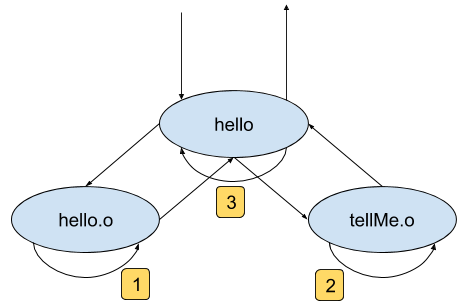
\includegraphics[width=0.6\textwidth]{figures/SOP_s04_ex4_c_1}
    }
  \caption{\label{fig:ex4-1}Execution tree of $(1)$.}
\end{figure}

\begin{figure}[ht]
  \centering
  \frame{
  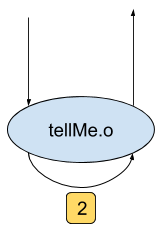
\includegraphics[width=0.2\textwidth]{figures/SOP_s04_ex4_c_3}
    }
  \caption{\label{fig:ex4-3}Execution tree of $(3)$.}
\end{figure}

\begin{figure}[ht]
  \centering
  \frame{
  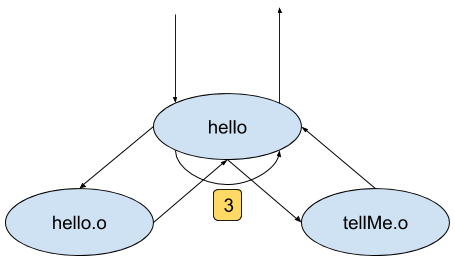
\includegraphics[width=0.6\textwidth]{figures/SOP_s04_ex4_c_4}
    }
  \caption{\label{fig:ex4-4}Execution tree of $(4)$.}
\end{figure}

\begin{figure}[ht]
  \centering
  \frame{
    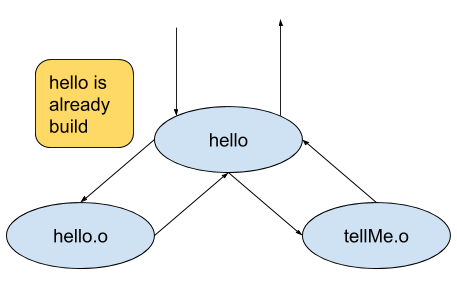
\includegraphics[width=0.6\textwidth]{figures/SOP_s04_ex4_c_5}
    }
  \caption{\label{fig:ex4-5}Execution tree of $(5)$.}
\end{figure}

\subsection*{d)}

\subsubsection{\texttt{tellMe\_unwiseBug.c}}

There is no problem at the compilation or at running time.

\subsubsection{\texttt{tellMe\_compBug.c}}

There is an error at the compilation, because the function $tellMe$ is declared
with two differents signatures. Once, it has an argument of type $char$ and
another time it is declared with argument of type $char[]$ (pointer of char).

\subsubsection{\texttt{tellMe\_execBug.c}}

There is no problem at the compilation. At the running time, the problem is that
$tellMe$ is called with an incorrect argument (wrong type). The problem appears
because we don't check function prototypes across compiled source files.

\end{document}
